\documentclass[../../main.tex]{subfiles}
 
\begin{document}

\section{Лекция 6. 21 ноября 2019 г.}


Вспомним материалы прошлой лекции:

$(X, \tau)$ - топологическое пространство, $Y \subset X$

$\tau_Y= \left\{U \cap Y \colon U \in \tau \right\}$ - \textit{индуцированная} топология на $Y$.

$i_Y \to x$ - отображение включения. $i_Y(y) = y \; \fo y \in Y$

$\tau_Y$ - самая грубая топология на $Y$, в которой $i_Y$ непрерывно

$f \colon X \to Y$ - отображение множеств, $A \subset X$

\defn \textit{Ограничение} $f$ на $A$ - это  $f|_A \colon A \to Y, \: (f|_A)(a) = f(a) \; \fo a \in A$

\textbf{Предложение.} $X,Y$ - топологические пространства, $A \subset X,\; f \colon X \to Y$ непрерывно $\Ra f|_A \colon A \to Y$ непрерывно

\textit{Доказательство:} $f|_A = f \circ i_a \quad \square$

\textbf{Предложение:} 

(1) Множество $B \subset Y$ замкнуто в $\tau_Y \lra B = F \cap Y$ для некоторого замкнутого $F \subset X$

(2) $\fo A \subset Y$ (замыкание $A$ в $(Y, \tau_Y))  = \overline{A} \cap Y$, где $\overline{A}$ - замыкание $A$ в $X$. 

\textit{Доказательство:} (1) следует из формулы $Y \backslash B = (X \backslash B) \cap Y \;\; \fo B \subset Y$

(2) (Замыкание $A$ в $X$) $ = \bigcap \left\{C \subset Y \colon C \; замкнуто \; в \; (Y, \tau_Y) и \; C \supset A \right\} =^{(1)} \cap \left\{F \cap Y \colon F\; замкнуто \; и \; F \supset A \right\}  =   $

$= \left( \cap \left\{ F \colon F \; замкнуто \; в \; X и \; F \supset A \right\} \right) \cap Y = \overline{A} \cap Y \quad \square$

\textit{Предложение:} $X$ - топологическое пространство, $A \subset Y \subset X$

(1) Если $Y$ открыто в $X$, то $A$ открыто в $Y \lra A$ открыто в $X$

(2) Если $Y$ замкнуто в $X$, то $A$ замкнуто в $Y \lra A$ замкнуто в $X$

\textit{Доказательство:} (1) $\Ra A = Y \cap U$, где $U$ открыто в $X \Ra A$ открыто в $X$

$(\Leftarrow) A = Y \cap \underbrace{A}_{открыто \; в\; x} \Ra A$ открыто в $Y$

(2) Аналогично. $\quad \square$

\subsection{Инициальные топологии. Произведения топологических пространств.}

1 \textit{Инициальные топологии}

$X$ - множество, $(X_i, \tau_i)_{i \in I}$ - семейство топологических пространств $(I \neq \varnothing); \; (f\colon X \to X_i)_{i \in I}$ - семейство отображений.

\defn \textit{\textbf{Инициальная топология}} на $X$, порожденная семейством $(f_i)_{i \in I}$ - это топология $\tau_{in}$ на $X$ с предбазой $\left\{ f^{-1}_i(U) \colon i \in I, U \in \tau_i \right\}$

\textbf{Пример 1.} $X$ - топологическое пространство, $Y \subset X$

Индуцированная топология на $Y = $ инициальная топология, порожденная $\left\{ i_Y \colon Y \to X \right\}$

\textit{Обозначение:} $\pt$ - топологическое пространство, состоящее из одной точки. (от слова point)

\textbf{Пример 2.} $X$ - множество. Инициальная топология на $X$, порожденная $\left\{X \to \pt \right\}$ - антидискретная топология.

\textbf{Теорема} (основные свойства инициальной топологии)



\begin{minipage}{0.15\linewidth}
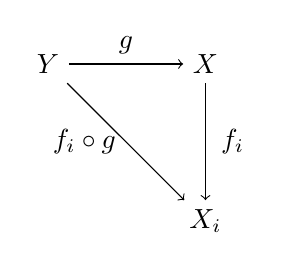
\begin{tikzpicture}[node distance=2cm, auto]
\node (Y) {$Y$};
\node(X) [right of=Y] {$X$};
\node (X1) [below of=X] {$X_i$};
\draw[->](Y) to node {$g$}(X);
\draw[->](Y) to node [left] {$f_i\circ g$}(X1);
\draw[->](X) to node [right=0.5ex] {$f_i$}(X1);
\end{tikzpicture}
\end{minipage}
\begin{minipage}{0.85\linewidth}
$X$ - множество, снабженное инициальной топологией, порожденной семейством $(f_i \colon X \to X_i)_{i \in I}$

(1) $\tau_{in}$ - самая грубая топология на $X$, в которой все $f$ непрерывны,

(2) Если $Y$ - топологическое пространство, то отображение $g \colon Y \to X$ непрерывно $\lra f_i \circ g \colon Y \to X_i$ непрерывно $\fo i$.
\end{minipage}



\textit{Доказательство:} (1) $\fo i \in I \; \fo U \in \tau_i \quad f^{-1}_i (U) \in \tau_{in} \Ra f_i$ непрерывно.

Пусть $\sigma$ - некоторая топология на $X$, т.ч. $\fo i \in U \quad f_i \colon (X, \sigma) \to X_i$ непрерывно

$\fo i \in I \; \fo U \in \tau_i \quad f^{-1}_i(U) \in \sigma \Ra (предбаза \; \tau_{in}) \subset \sigma \Ra \tau_{in} \subset \sigma$

(2) $(\Ra)$ Если $g$ непрерывно, то $f_i \circ g$ непрерывно, т.к. $f$ непрерывно

$(\Leftarrow)$ Пусть $f_i\circ g$ непрерывно $\fo i$

Достаточно доказать: $\fo $ множества $V \subset X$ из предбазы $\tau_{in} \quad g^{-1}(V)$ открыто в $Y$

$V = f^{-1}_i(U)$, где $U \subset X$ открыто $\Ra g^{-1}(f^{-1}_i(U)) = (f_i \circ g)^{-1}(U)$ - открыто в $Y \;\; \square$

\textit{Упражнение} $\tau_{in}$ - единственная топология на $X$ со свойством (2).

\subsection{Произведения множеств}

$(X_i)_{i \in I}$ - семейство множеств.

\defn \textit{Произведение} семейства $(X_i)_{i \in I}$ - множество:

$$\prod_{i \in I} X_i = \left\{ x \colon I \to \bigcup_{i \in I} X_i \Big| \fo i \in I \; x(i) \in X_i \right\}$$

\textit{Частный случай} Если $X_i = Y \fo i$, то $\prod_{i \in I}X_i = Y^{I}$ - множество всех отображений $I \to Y$

\textit{Обозначения.} $\fo x \in \prod_{i \in I} X_i \;\; x_i = x(i), \;\; x = (x_i)_{i \in I} \;\; (x_i \in X_i)$

Если $I = \{1, \ldots, n \}$, то вместо $\prod_{i \in I}X_i$ пишут $\prod^{n}_{i = 1} X_i$ или $X_1 \times X_2 \times \ldots \times X_n$

В этом случае элементы $X_1 \times X_2 \times \ldots \times X_n$ - упорядоченные наборы $(x_1, \ldots, x_n)$, где $x_i \in X_i$.

\textit{Обозначение.} $\fo j \in I \;\; p_J \colon \prod_{i \in I} X_i \to X_j, \;\; p_j(x) = x_j$

$p_j$ - \textit{каноническая проекция} на $X_j$

\subsection{Произведения топологических пространств}

$(X_i, \tau_i)_{i \in I}$ - семейство топологических пространств, $X = \prod_{i \in I} X_i$

\defn \textit{\textbf{Топология произведения}} (\textit{тихоновская топология}) на $X$ - это инициальная топология, порожденная семейством $\left\{p_j \colon X \to X_j \right\}_{j \in I}$ канонических проекций.

\textit{Наблюдение:} (1) $\fo$ открытого $U \subset X_i$

$p^{-1}_i(U) = \prod_{j \in J}$, где $V_j = \begin{cases} U\; при \; j = i \\ X_j \; при \; j \neq i \end{cases}$. Множества вида (1) образуют предбазу $X$.

(2) $\fo$ конечного $I_0 \subset I, \; \fo i \in I_0$ пусть $U_i \subset X_i$ - открытое множество.

(**) $\bigcap_{i \in I_0} p^{-1}_i (U_i) = \prod_{j \in I}V_j,$ где $V_j =\begin{cases} U_j\; при \; j \in I_0 \\ X_j \; при \; j \notin I_0 \end{cases} $

Множества вида (**) образуют базу $X$.

(3) Если $I$ конечно, то базу $X$ образуют множества вида $\prod_{i \in I} U_i$, где $U_i \subset X_i$ открыто.

\textbf{Предостережение-упражнение:} Если $I$ бесконечно, то $\prod_{i \in I} U_i$ не обязательно открыто в $X$ (где $U_i \subset X_i$ открыто)

\textit{Отступление:} коммутативные диаграммы

(здесь будут картинки диаграмм)

\textbf{Теорема} (универсальное свойство произведения)

$(X_i)_{i \in I}$ - семейство топологических пространств, $X = \prod_{i \in I}X_i,\; p_i \colon X \to X_i$ - каноническая проекция; $Y$ - топологическое пространство.

\begin{minipage}{0.15\linewidth}

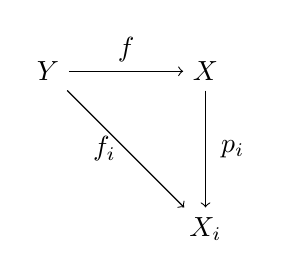
\begin{tikzpicture}[node distance=2cm, auto]
\node (Y) {$Y$};
\node(X) [right of=Y] {$X$};
\node (X1) [below of=X] {$X_i$};
\draw[->](Y) to node {$f$}(X);
\draw[->](Y) to node [left] {$f_i$}(X1);
\draw[->](X) to node [right=0.5ex] {$p_i$}(X1);
\end{tikzpicture}

\end{minipage}
\begin{minipage}{0.80\linewidth}
Тогда для любого семейства $(f_i \colon Y \to X_i)_{i\in I}$ непрерывных отображений $\ex!$ непрерывное отображение $f \colon Y \to X_i$, такое что диаграмма (D) коммутативна $\fo i \in I$
\end{minipage}

\textit{Доказательство:} Определим $f \colon Y \to X$ так: $\left( f(y) \right)_i = f_i(y) \; \fo y \in Y, \fo i \in I$

Отображение $f$ делает диаграмму (D) и является единственным отображением с этим свойством. Его непрерывность следует из теоремы о свойствах инициальной топологии. $\quad \square$.

\textit{Предложение.} $(X_i, \ro_i) \; (i = 1, \ldots, n)$ - метрические пространства, $X = \prod^n_{i = 1}X_i$

Определим $\ro\colon X \times X \to [0, +\infty)$ так: $\ro(x,y) = \max_{1 \leq i \leq n}\ro_i(x_i, y_i)$

Тогда $\ro$-метрика на $X$, и она порождает топологию на $X$.

\textit{Доказательство:} Упражнение: $\ro$ - метрика.

Обозначим $\tau = $ топология произведения на $X, \tau_{\ro}$ - тополония, порожденная $\ro$.

Заметим: $\ro(x, y) < r \lra \ro_i(x_i, y_i) < r \; \fo i = 1, \ldots, n $

$(\Ra) B_r(x) = \prod^n_{i = 1}B_r(x_i) \Ra B_r(x)$ открыто в $\tau \Ra \tau_{\ro} \subset \tau$

Пусть $U$ - множество из базы $\tau$; $U = \prod^n_{i = 1}U_i$, где $U_i \subset X_i \fo i$ открыто

Пусть $x \in U$. Тогда $\fo 1 = 1, \ldots, n \;\; x_i \in U_i \Ra \ex r_i > 0 \colon B_r(x) \subset U_i$

Обозначим $r = \min_{1 \leq i \leq n} r_i \lra B_r(x) \prod^n_{i = 1} B_r(x_i) \subset  \prod^n_{i = 1} B_{r_i}(x) \subset  \prod^n_{i = 1} U_i = U$

$\Ra U$ открыто в $\tau_{\ro} \Ra \tau \subset \tau_{\ro} \Ra \tau = \tau_{\ro} \;\; \square$

\textit{Следствие:} $\K = \R$ или $\mathbb{C}$

Стандартная топология на $\K^n$, порожденная $||\cdot||_{\infty}$ (или $||\cdot||_1$ или $||\cdot||_2$) совпадает с топологией произведения $\K \times \K \times \ldots \times \K$.



\end{document}